\section{Etapa de Ejecuci\'on}
Esta etapa se encarga de las operaciones entre los datos que vienen desde el latch, como se ve en la figura 

\begin{figure}[H]
\centering
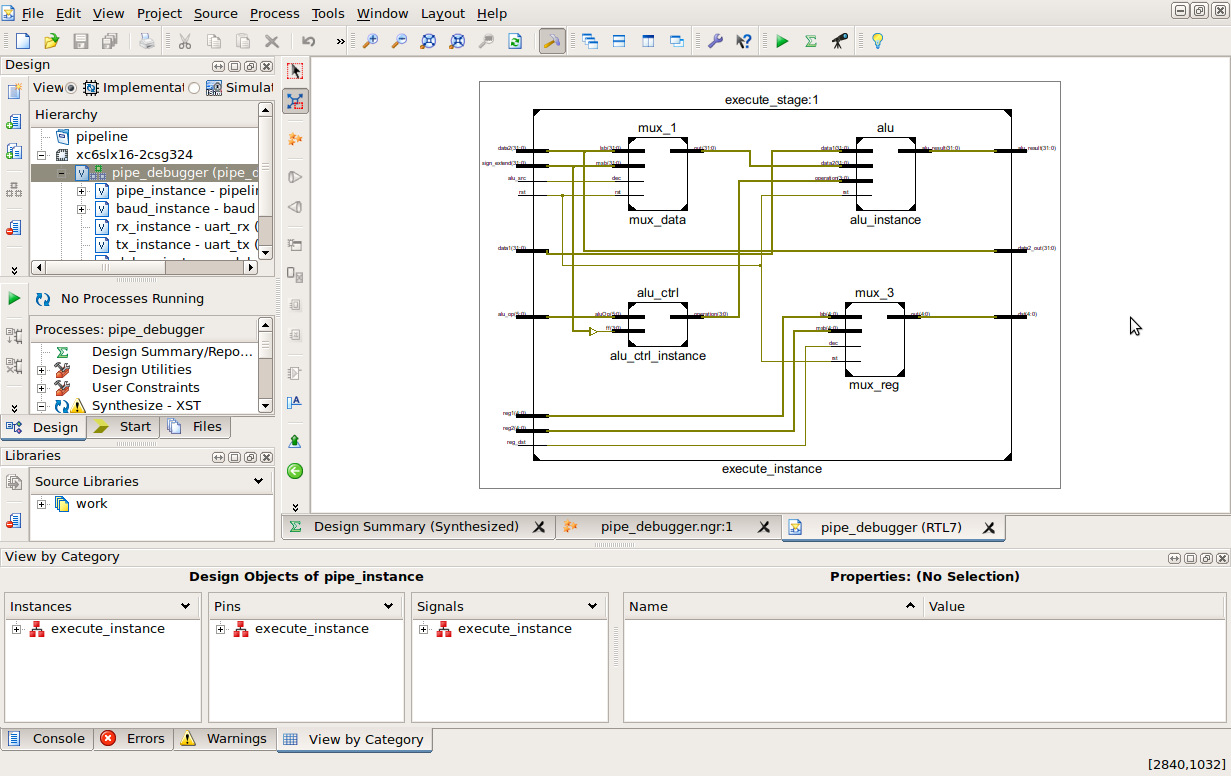
\includegraphics[scale=0.5]{img/execute_stage_inside}
\caption{Etapa de ejecuci\'on}
\label{fig:fetch}
\end{figure}

Esta etapa se encarga de operar con los datos que se le presentan en la entrada, eligiendo la operaci\'on que fue decodificada en la etapa anterior y pasando el resultado a la siguiente etapa.
Tiene como entradas:

\begin{itemize}
  \item \textbf{alu\_op}: Bus de 6 bits que lleva los datos para que la unidad de control de la alu se encargue de elegir que operacion ejecutar.	
  \item \textbf{data1}: Datos que entran a la alu para ser procesados.
  \item \textbf{data2}: Datos que entran en el mux1 para elegir contra sign\_extend y tambien sale directamente hacia el latch.
  \item \textbf{reg1}: entra a mux\_2 para elegir contra reg2 segun la senal reg\_dst para conocer cual de los registros se va a escribir en el banco de registros en la etapa de escritura.
  \item \textbf{reg2}: entra a mux\_2 para elegir contra reg1 seg\'un la senal reg\_dst para conocer cual de los registros se va a escribir en el banco de registros en la etapa de escritura. 	
  \item \textbf{sign\_extend}: Extensi\'on de signo que entra en el multiplexor mux\_1 para elegir contra data2 y entrar a la alu para operar.
  \item \textbf{alu\_src}: Senal que elige entre data2 y sign\_extend en el mux\_1
  \item \textbf{reg\_dst}: Senal que elige entre uno de los dos registros en mux\_2 que entran a la etapa para conocer cual se escribe en la etapa de escritura.
  \item \textbf{rst}: Reinicio del m\'odulo. 
\end{itemize}

Tiene los modulos alu, alu\_ctrl y dos multiplexores.

\subsection{Control de la ALU}
El control de la alu en detalle se muestra en la siguiente figura.

\begin{figure}[H]
\centering
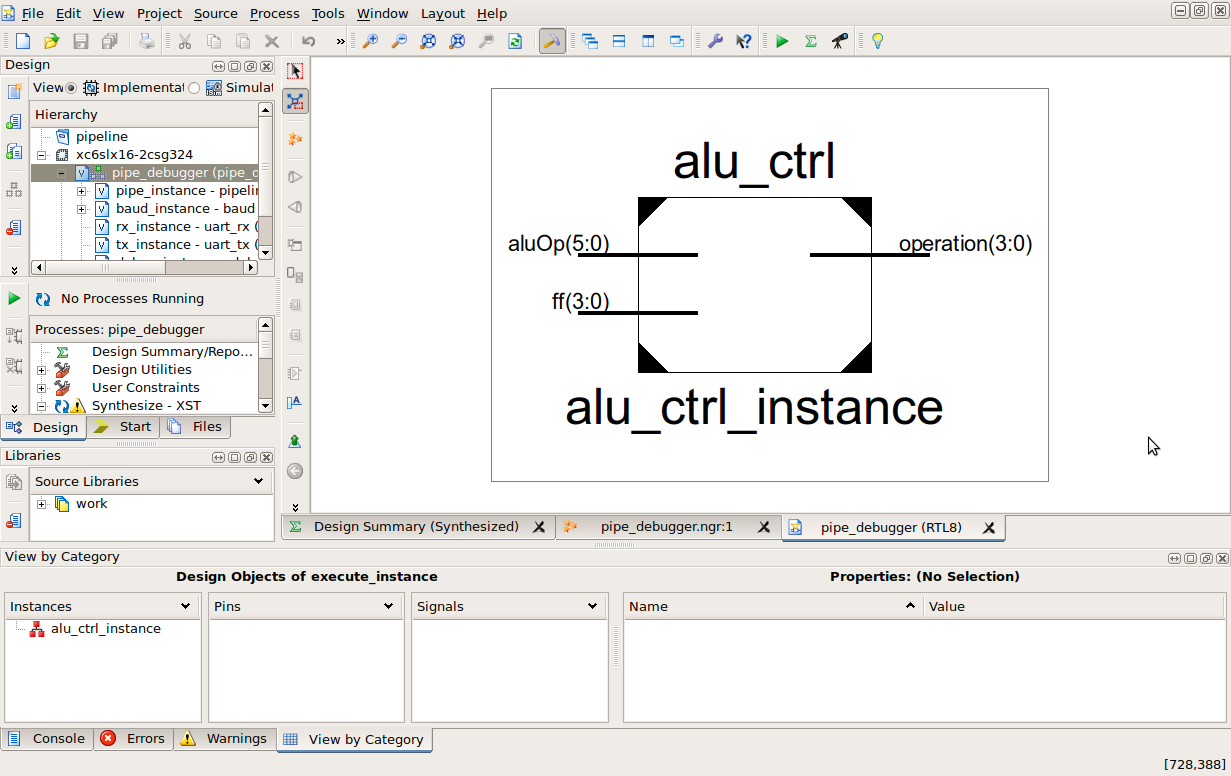
\includegraphics[scale=0.5]{img/alu_ctrl}
\caption{M\'odulo de control de la ALU}
\label{fig:fetch}
\end{figure}

Tiene como entradas:

\begin{itemize}
  \item \textbf{alu\_op}: Opcode que entra a este m\'odulo para decodificar que operaci\'on debe realizar la alu.
  \item \textbf{ff}: Entran 4 bits que provienen de la parte baja extensi\'on de signo y genera el opcode que utiliza la alu para ejecutar la operaci\'on.  
\end{itemize}

Y la salida:
\begin{itemize}
  \item \textbf{operation}: Bus de 4 bits que ingresa a la alu para realizar la operaci\'on correspondiente.
\end{itemize}

\subsection{ALU} 
La ALU es el coraz\'on de esta etapa y es la que se encarga de sumar ejecutar la operacion correspondiente a los operandos suministrados.

\begin{figure}[H]
\centering
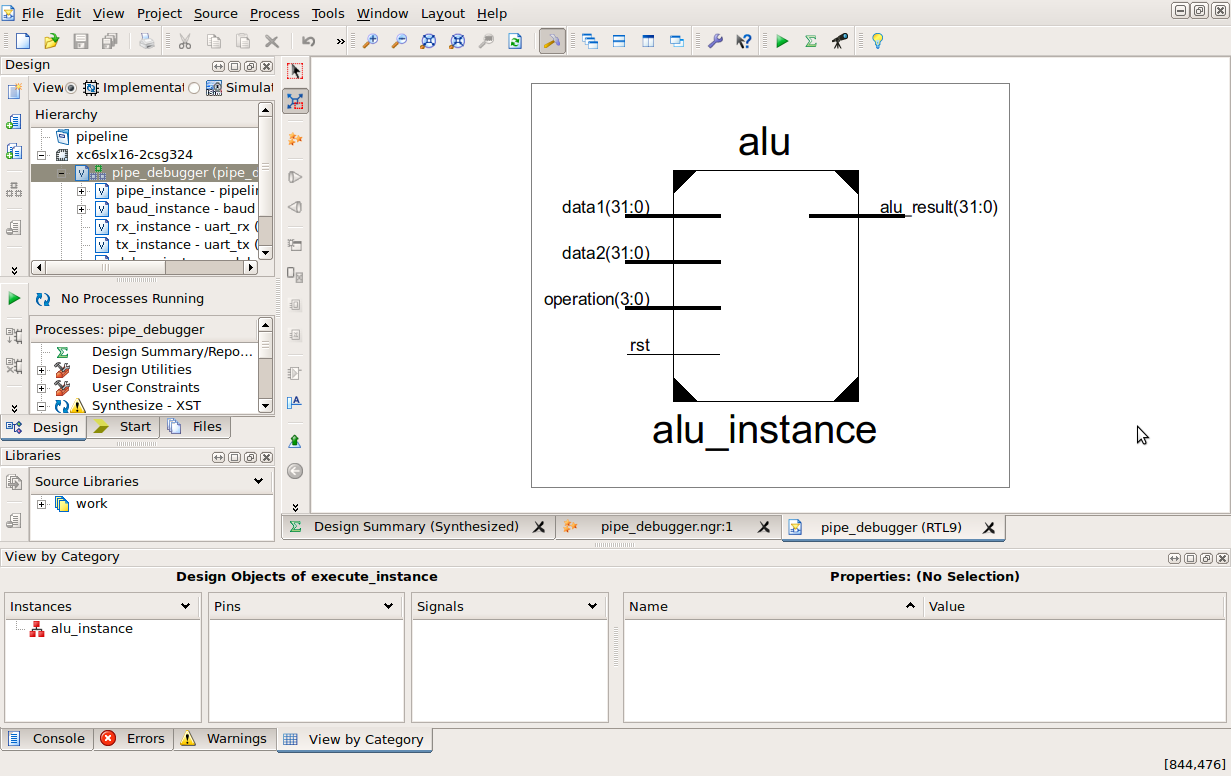
\includegraphics[scale=0.5]{img/alu}
\caption{ALU}
\label{fig:fetch}
\end{figure}

Entradas:

\begin{itemize}
  \item \textbf{data1}: Primer operando.
  \item \textbf{data2}: Segundo operando.
  \item operation: Operaci\'on a realizar con los operandos dentro del m\'odulo.
  \item \textbf{rst}: Señal de reset del m\'odulo.
\end{itemize}

Salida:

\begin{itemize}
  \item \textbf{alu\_result}: Resultado de la operaci\'on realizada entre los operandos.
\end{itemize}

\begin{center}
\begin{table}[H]
%\resizebox*{15cm}{!}{
\scriptsize
\centering
\begin{tabular}[\textwidth]{|l|l|}
\hline
AND & 0000\\
\hline
OR & 0001\\
\hline
SUMA & 0010\\
\hline
XOR & 0100\\
\hline
NOR & 0101\\
\hline
Branch EQUAL & 0110\\
\hline
XOR Inmediato & 1001\\
\hline
SLT & 0111\\
\hline
\end{tabular}
\center
\caption{Tabla de operaciones de la ALU}
\label{tab:test1}
\end{table}
\end{center}

\subsection{Testbench}